\section{This chapter has a very long title that would be too long for using in headers and table of contents}

Given the vastness of the field of Image Processing, this document will not attempt to provide a comprehensive overview of the subject as a whole. Instead, only those areas that are specifically pertinent to the project at hand will be covered. It is worth noting that this document includes cross-referencing to other sections, such as Section 2.2, to provide additional context and understanding.
\medskip % needed for paragraph separation
\newline % needed for paragraph separation
Here is an illustration of a list with bullet points:
\begin{itemize}
    \item Mean: The mean value of the neighborhood is calculated.
\end{itemize}

\noindent Here is one mathematical equations:
\medskip % needed for paragraph separation
\newline % needed for paragraph separation
$\mu = \frac{\sum_{i=1}^{n} x_i}{n}$
\medskip % needed for paragraph separation
\newline

\section{Analysis of Results}

\noindent
\blindtext
\medskip
\newline

\begin{table}[!ht]
    \centering
    \begin{tabular}{|c|c|}
    \hline
        \multicolumn{2}{|c|}{Personal Computer (VMWare's Virtual Machine)} \\ \hline
        Brand & MSI \\ \hline
        Operating System & Linux (Ubuntu 22.04) \\ \hline
        Processor & Intel(R) Core(TM) i7-9750H \\ \hline
        Cores & 8 \\ \hline
        RAM Memory & 16 GB \\ \hline
    \end{tabular}
    \caption{Specifications of the machine on which the tests have been made}
\end{table}
\noindent \blindtext
\newline

\begin{figure*}[!ht]
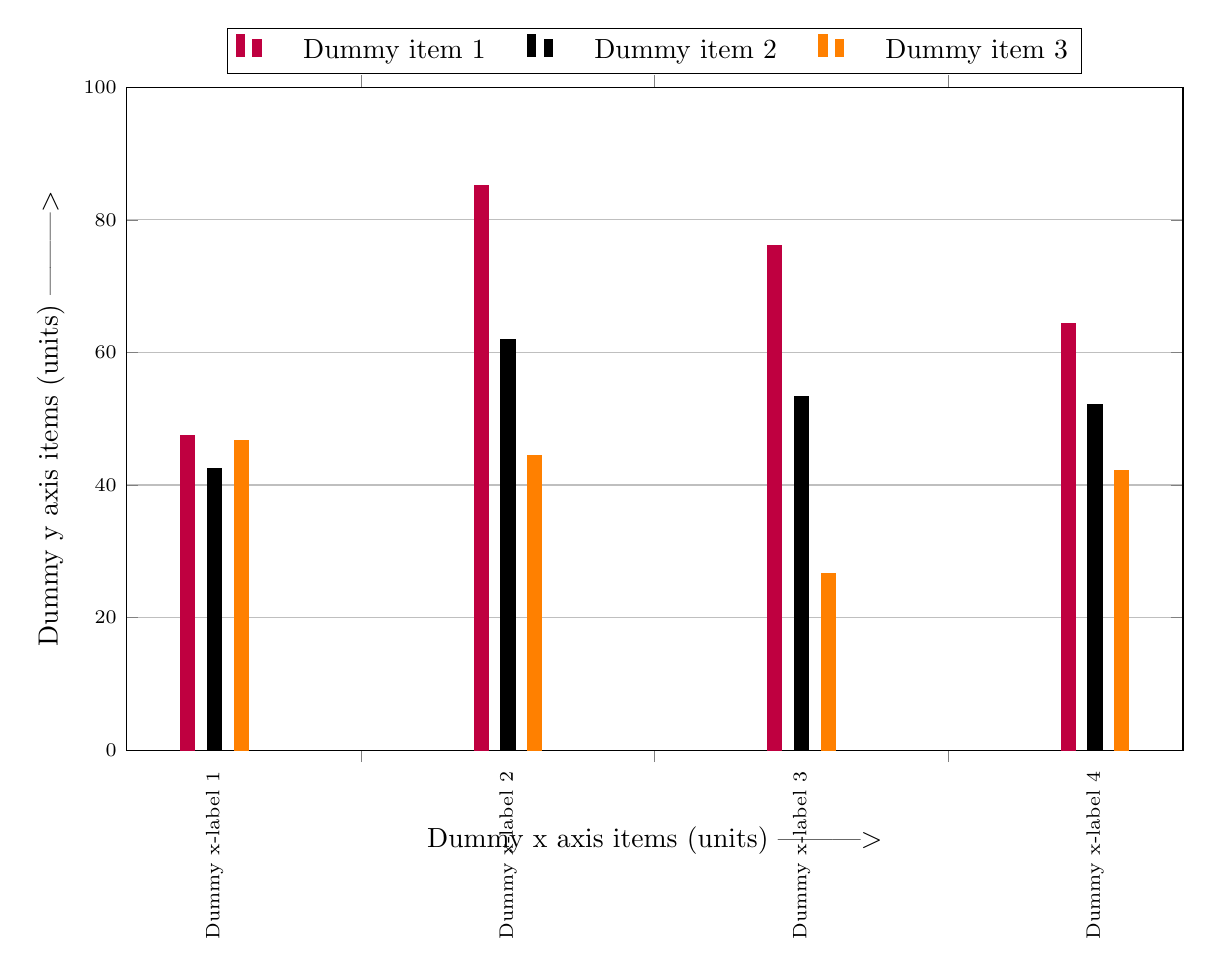
\begin{tikzpicture}
    \begin{axis}
        [ybar=0.16cm,
        bar width=0.18cm,
        width=15cm,
        height=10cm,
        ymin=0,
        ymax=100, % if your chart goes for a major value of y axis, you just change this line
        yticklabel style={font=\scriptsize},
        xtick=data,
        xticklabels={Dummy x-label 1, Dummy x-label 2, Dummy x-label 3, Dummy x-label 4}, % if you want more x axis columns, you just have to put one more item in here
        xticklabel style={yshift=0ex, rotate=90, font=\scriptsize},
        x label style={at={(axis description cs:0.5,-0.1)},anchor=north},
        xlabel={Dummy x axis items (units) ---------{$>$}}, % if you want to check the x axis label you have to change the text in here
        ylabel={Dummy y axis items (units) ---------{$>$}}, % if you want to check the y axis label you have to change the text in here
        major x tick style={opacity=0},
        minor x tick num=1,
        minor tick length=1 ex,
        ymajorgrids= true,
        legend style={
            at={(0.50,1.02)},
            anchor=south,
            column sep=3ex,
            legend columns=-1,
        }
        ]

\addplot [style={purple, fill=purple}] coordinates {
    % if there is some more columns, you have to add one more item in here with last following number and add one to do another 
    (1,\num{47.445}) 
    (2,\num{85.153}) 
    (3,\num{76.153}) 
    (4,\num{64.412})
};
\addplot [style={black, fill=black}] coordinates {
    (1,\num{42.429}) 
    (2,\num{62.020}) 
    (3,\num{53.341}) 
    (4,\num{52.207})
};

\addplot [style={orange, fill=orange}] coordinates {
    (1,\num{46.665}) 
    (2,\num{44.440}) 
    (3,\num{26.685}) 
    (4,\num{42.139})
};

% if you want more item columns, you have to add the previos \addplot in here and change the color

    \legend{Dummy item 1, Dummy item 2, Dummy item 3};
    \end{axis}
\end{tikzpicture}
    \centering
      
    \caption{ Dummy Grouped Bar Chart }
    \label{fig:my_label}
\end{figure*}

\newpage